\chapter{Implementation}
\label{chap:implementation}
This chapter highlights the implementational aspects of the system. Introducing the technologies used to build the components. Each section title refers to its respective GitHub repository of the \texttt{ARTIS-project}\footnote{\href{https://github.com/artis-project/}{https://github.com/artis-project/}} GitHub organization.

\section{artis-smartcontract}
The \gls{sc} was written in Ethereum's native programming language Solidity \cite{solidity}. The contract was developed using hardhat \cite{hardhat}, a development environment for Ethereum. Hardhat makes developing, compiling, testing, and deploying smart contracts easy. The \gls{sc} has been deployed to the Ethereum testnet Sepolia \cite{sepolia} during development but is intended to be deployed on the mainnet in production. The Ethereum blockchain was selected due to the research group's and the author's prior experience.

When the \gls{sc} is first deployed the \texttt{smartcontractAdmin} variable is set to the deploying address. This address will be the only point of access to any \gls{sc} function. It is also the account used by the server to interact with the \gls{sc} and sign transactions.

\lstinputlisting[
    language=Solidity,
    caption=\gls{sc} constructor function,
    label=lst:scconstructor,
    firstline=53,
    lastline=55
]{codesnippets/smartcontract.sol}

As seen in Listing \ref{lst:scconstructor} the \gls{sc} extends the ERC721 \cite{erc721} contract which provides the \gls{nft} interface.

\subsection{Data Structures and Events}
We will explain the data structures used in more detail to understand the rest of the contract.

\subsubsection{Structs}
To satisfy the artwork tracking use case three additional structs have been defined as seen in Listing \ref{lst:scstructs}. The \texttt{ArtworkData} struct contains all information about a specific artwork. This includes the addresses of each actor as well as the violation timestamp and the status of the artwork. The status field in turn contains two fields as defined in the \texttt{Status} struct. They are used to support the multi-approval process when it comes to changing the status of an artwork. To match the physical artwork with the \gls{nft} we also included an objectID field. If needed, the \texttt{ArtworkData} struct can be extended with more data fields.

The \texttt{StatusApprovals} struct stores which of the actors has already approved a status change. The logic behind this multi-approval process will be explained in detail later.

\lstinputlisting[
    language=Solidity,
    caption=\gls{sc} structs,
    label=lst:scstructs,
    firstline=1,
    lastline=20
]{codesnippets/smartcontract.sol}

\subsubsection{Enums}
The \gls{sc} defines one enum that defines the different status values that exist. Enums help during development as they prevent misspellings or other types of errors.

\lstinputlisting[
    language=Solidity,
    caption=\gls{sc} enums,
    label=lst:scenums,
    firstline=22,
    lastline=27
]{codesnippets/smartcontract.sol}

\subsubsection{Mappings}
The \texttt{artworks} mapping is used to map artwork ids to \texttt{ArtworkData} structs. This mapping is used to store the references to each new artwork. Similarly, the \texttt{approvals} mapping is used to store and manage the approval data of an artwork. Simply put, this mapping can answer the question of who has approved a certain status of a specific artwork.

\lstinputlisting[
    language=Solidity,
    caption=\gls{sc} mappings,
    label=lst:scmappings,
    firstline=29,
    lastline=32
]{codesnippets/smartcontract.sol}

\textit{e.g.} \texttt{approvals[1][StatusValue.IN\_TRANSIT].carrier} is \texttt{true} if and only if the carrier has already approved to change the artwork status of artwork $1$ to IN\_TRANSIT.

\subsubsection{Events}
The contract defines three events (Listing \ref{lst:scevents}). The \texttt{Updated} event is emitted whenever the data associated with an artwork has changed. The \texttt{StatusApproved} event is emitted whenever the multi-approval process (Figure \ref{fig:update_status}) has been successful. If an approval is still missing the \texttt{ApprovalMissing} event is emitted. Users can subscribe to these events and be notified whenever an event is emitted.

\lstinputlisting[
    language=Solidity,
    caption=\gls{sc} events,
    label=lst:scevents,
    firstline=171,
    lastline=188
]{codesnippets/smartcontract.sol}

\subsection{Functions and Modifiers}
To support the functionality designed in Section \ref{sec:overview} the contract implements three main functions, modifiers, and helper functions. However, we will not go into detail about the helper functions.

\subsubsection{Function Modifiers}
In Solidity, we can define function modifiers, that can be used to prepend functionality to a function. If a function modifier is used in a function the code in the modifier is executed beforehand. For instance, this can be used to perform a check before a function is run. Function modifiers can be reused on multiple functions and thus introduce cleaner and less redundant code.

\lstinputlisting[
    language=Solidity,
    caption=\gls{sc} modifiers,
    label=lst:scmodifiers,
    firstline=81,
    lastline=121
]{codesnippets/smartcontract.sol}

The modifiers in Listing \ref{lst:scmodifiers} are used to check if a caller is authorized to call a specific function. If the call is forbidden the transaction is reverted with an appropriate error message. The last three characters of each error message represent the corresponding \gls{http} status code. This status code is directly forwarded by the server \gls{api} in case of an error.

To ensure that all \gls{sc} interaction is done through the server \gls{api} we modified every public function with the \texttt{onlyAdmin} modifier. This modifier reverts any transaction which is sent from a different account than the specified admin account.

The \texttt{read} modifier is additionally added to each function that reads data from the \gls{sc}. We check that the wallet that authenticated a request to the server \gls{api} is registered as an actor with read permissions.

Similarly, we defined the \texttt{write} modifier to check that certain \texttt{ArtworkData} fields are only modified by the owner or logger respectively. The \texttt{currentStatus} field cannot be modified at all, it is updated automatically once the actors approved a status change. The detailed permission sets of each actor can be found in Table \ref{tab:permission_sets}

The contract makes use of one additional modifier called \texttt{exists} which simply checks if a given tokenId exists.

\subsubsection{safeMint}
This function is called to create a new \gls{nft}. This process is called "minting". The safeMint function in an ERC721 contract creates and assigns ownership of a new \gls{nft} to a designated recipient. 

\lstinputlisting[
    language=Solidity,
    caption=\gls{sc} safeMint function,
    label=lst:scsafemint,
    firstline=139,
    lastline=148
]{codesnippets/smartcontract.sol}

Our implementation is rather straightforward, first, we increment the counter variable, which keeps track of the total supply. We also use this number as a token identifier which is equal to the artwork \gls{id}. With this unique \gls{id}, we call the \texttt{\_safeMint(to, tokenId)} function of the ERC721 contract provided by openzeppelin \cite{openzeppelin}. In Line 8 of Listing \ref{lst:scsafemint}, we initialize a new ArtworkData instance with the initial data, which is partially provided by the user via a function parameter. We assign the values of the objectID property, the actors, and the logger properties. The violation timestamp, \gls{id}, and status properties are ignored and set to a default value. Finally, the artwork data is associated with the newly minted artwork in the \texttt{artworks} mapping.

\subsubsection{updateArtworkData}
The data associated with an artwork can be updated by calling this function. Upon successful update, the function does not return anything but emits an event with the updated values. This is based on a limitation of Solidity where it is impossible to return an object from a state-changing function. Additionally, this function allows you to update multiple fields at once. This has some advantages:

\begin{itemize}[align=left, font=\itshape]
    \item[simplified interface:] Using only one update function instead of exposing an update function for each field reduces the number of public functions. This results in a more understandable and usable contract.
    \item[atomic updates:] If an error occurs during the execution of this function the transaction as a whole is reverted, resulting in the initial state of the contract. This maintains data consistency and prevents partial updates.
    \item[reduced costs:] The possibility to update multiple fields at once reduces the number of transactions that need to be submitted and in turn reduces execution costs.
\end{itemize}

\lstinputlisting[
    language=Solidity,
    caption=\gls{sc} updateArtworkData function,
    label=lst:scupdate,
    firstline=123,
    lastline=137
]{codesnippets/smartcontract.sol}

The \texttt{updateArtworkData} expects the updated data as a parameter of the type ArtworkData. Solidity expects every field of the \texttt{data} parameter to be populated. This is why we check for each field if the value should be updated and execute the according update. For string fields, this check is done by checking the length of the incoming string. An empty string with length $0$ indicates that the user did not update this field. The same check is not possible with addresses. This is why we used the address $0$x$00...001$ to mark an empty address update field. The zero address $(0$x$0)$ is reserved to remove an address from a field.

The code to update artwork properties differs in complexity. For the \texttt{violationTimestamp} field it is as simple as assigning the new timestamp to the corresponding artwork: 
\begin{lstlisting}[language=Solidity]
    artworks[data.id].violationTimestamp = data.violationTimestamp
\end{lstlisting}
This works identically for updating the roles and the objectID. When updating the logger address we implemented an additional check to prevent updates when the artwork is IN\_TRANSIT.
\begin{lstlisting}[language=Solidity]
    require(
        !(artworks[data.id].status.currentStatus.equal("IN_TRANSIT")),
        "logger cannot be updated in transit 403"
    );
\end{lstlisting}

\paragraph{Updating the transportation status}
\label{sec:update_status}
The logic behind updating the status (Figure \ref{fig:update_status}) is more complex. The reason for this is the multi-approval feature of this contract. To satisfy our use case, the actors must agree on the transportation status of the artwork. To ensure this agreement, each affected actor must submit an update request with the same value. Only if this requirement is satisfied, is the binding transportation status updated. 

\begin{figure}[ht]
    \centering
    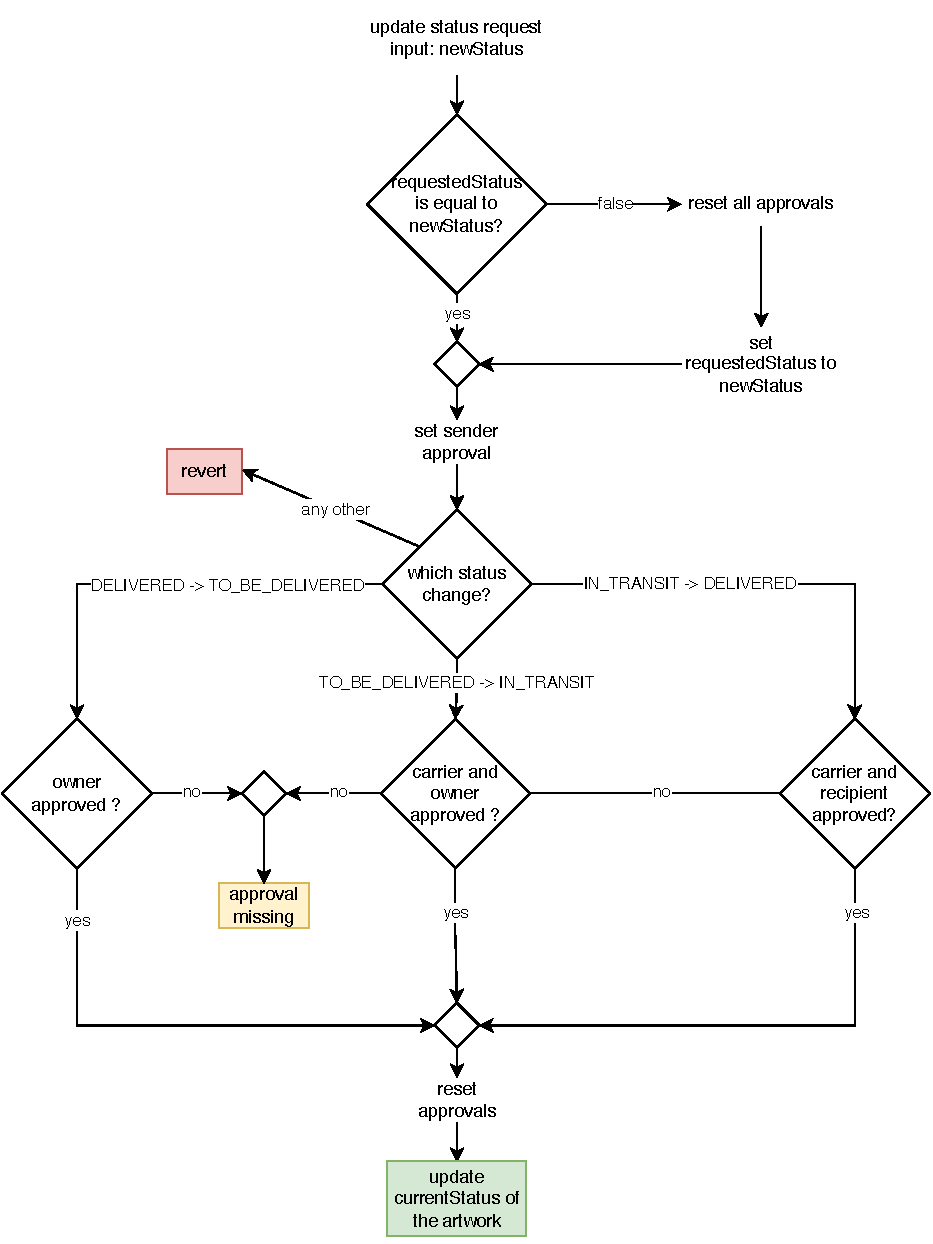
\includegraphics[height=0.62\textheight, keepaspectratio]{diagrams/update_status.drawio.pdf}
    \caption{Multi-approval transportation status change}
    \label{fig:update_status}
\end{figure}

To differentiate between the status that actors want to change to and the status which is currently in place we introduced two variables: \texttt{requestedStatus} and \texttt{currentStatus}. Users can request a status change by submitting a new \texttt{requestedStatus}. If this value does not match the previous value, all approvals are reset, and the \texttt{requestedStatus} field is set to the new value. The next step is to set the approval for the actor who sent the initial update request. Because different actors must approve different status changes, we must check for the three distinct cases.

If the status is requested to change from TO\_BE\_DELIVERED to IN\_TRANSIT, the carrier, and the owner must approve that change. This check is performed analogously for the change from IN\_TRANSIT to DELIVERED. Lastly, the owner decides to change from DELIVERED to TO\_BE\_DELIVERED. Any other combination of status changes is not allowed, and the transaction will be reverted.

If the right approvals have already been made, the function will automatically update the \texttt{currentStatus} and terminate. If any approval is missing, it will terminate without updating the \texttt{currentStatus}. In that case, the actor in question must submit their request for a status update.

\subsubsection{getArtworkData}
The function to retrieve data about an artwork is the simplest one. It merely returns the \texttt{ArtworkData} object mapped to the requested artwork \gls{id}. To easily convert the returned tuple to an object using the contract \gls{abi}, each property is mapped to the tuple entry specified in the function signature, visible in Listing \ref{lst:scget}.

\lstinputlisting[
    language=Solidity,
    caption=\gls{sc} getArtworkData function signature,
    label=lst:scget,
    firstline=150,
    lastline=169
]{codesnippets/smartcontract.sol}

\clearpage
\section{artis-server}
The server is the central part of the system; it connects the end users to the \gls{sc}. The responsibilities of the server can be separated into three layers. The files of the server's directory structure depicted in Figure \ref{fig:server_directory_structure} and the corresponding code will be explained in the next sections. The server code is implemented in Python using a variety of libraries that will be addressed later on.

\begin{figure}
    \centering
    \begin{forest}
  for tree={
    font=\ttfamily\footnotesize,
    grow'=0,
    child anchor=west,
    parent anchor=south,
    anchor=west,
    calign=first,
    edge path={
      \noexpand\path [draw, \forestoption{edge}]
      (!u.south west) +(7.5pt,0) |- node[fill,inner sep=1.25pt] {} (.child anchor)\forestoption{edge label};
    },
    before typesetting nodes={
      if n=1
        {insert before={[,phantom]}}
        {}
    },
    fit=band,
    before computing xy={l=15pt},
  }
[artis-server
    [/src
        [/authentication
            [Authenticator.py]
            [auth\_types.py]
        ]  
        [/models
            [Artwork.py]
            [Schemas.py]
            [Fields.py]
        ]
        [/smartcontract
            [ArtworkConnector.py]
            [SmartContractConnector.py]
        ]
    ]
    [/utils
        [error\_handlers.py]
    ]
    [app.py]
]
\end{forest}    
    \caption{Server directory structure}
    \label{fig:server_directory_structure}
\end{figure}

\subsection{Authentication Layer}
\label{sec:authentication_layer}
To implement the authentication flow described in section \ref{sec:authentication}, we defined an \texttt{Authenticator} class, which handles the server-side logic. This class implements functions provided by the third web library \cite{thirdweb} but has been adapted to fit our specific use case. The functionality described in this section is exposed by the \gls{api} via the endpoints listed in Table \ref{tab:authentication_endpoints}

\lstinputlisting[
    language=Python,
    caption=Generating the challenge payload,
    label=lst:authpayload,
    firstline=1,
    lastline=15,
    float
]{codesnippets/authenticator.py}

The method described in Listing \ref{lst:authpayload} constructs a dictionary with the information used to build the challenge message. The method is exposed by the \gls{api} layer via the \texttt{/auth/payload} endpoint as listed in Table \ref{tab:authentication_endpoints}. This dictionary is then returned to the client who constructs a message from it and signs it.

\lstinputlisting[
    language=Python,
    caption=Verifying the signature,
    label=lst:authlogin,
    firstline=17,
    lastline=32
]{codesnippets/authenticator.py}

The signed message is then sent back and verified by the \texttt{verify} method listed in Listing \ref{lst:authlogin}. After reconstructing the challenge message, the method recovers the account address that was used for the signature. If it matches the address specified in Line 7 of Listing \ref{lst:authpayload} the authentication request is valid. This proves that the user who sent the request has the specified account. To recover the address, the python web3 library was used \cite{web3python}.

If the authentication request succeeds the client will issue a \gls{jwt} signed by the server wallet. This token is then used to authenticate further requests until it expires. The \gls{jwt}'s signature and expiration date are verified upon each request by the \texttt{Authenticator} class. The \texttt{Authenticator} exposes this functionality with the \texttt{/auth/login} endpoint.

Two additional authentication endpoints are exposed by the \gls{api}. \texttt{/auth/logout} closes the session and \texttt{/auth/user} returns information about the subject of a \gls{jwt}. It can be queried to check if the session is still active and react accordingly on the client side.

\subsection{API Layer}
To expose the functionality defined in the use case and implemented in the \gls{sc}, it is enough to implement four different \gls{api} endpoints. The authentication mechanism described in Section \ref{sec:authentication_layer} provides another set of four endpoints.

\begin{table}[h]
    \begin{subtable}{0.45\textwidth}
        \centering
        \begin{tabular}{ll}
            \textbf{Endpoint}                    & \textbf{Method} \\ \hline
            \texttt{/artworks}                   & POST             \\
            \texttt{/artworks}                   & GET               \\
            \texttt{/artworks/<int:artwork\_id>} & GET                \\
            \texttt{/artworks/<int:artwork\_id>} & PATCH
        \end{tabular}
        \caption{Resource endpoints}
        \label{tab:resource_endpoints}
    \end{subtable}
    \hfill
    \begin{subtable}{0.45\textwidth}
        \centering
        \begin{tabular}{ll}
            \textbf{Endpoint}                       & \textbf{Method} \\ \hline
            \texttt{/auth/payload}               & POST                \\
            \texttt{/auth/login}                 & POST                 \\
            \texttt{/auth/logout}                & POST                  \\
            \texttt{/auth/user}                  & GET 
        \end{tabular}
        \caption{Authentication endpoints}
        \label{tab:authentication_endpoints}
    \end{subtable}
\caption{\gls{api} endpoints}
\end{table}

The \gls{json} schema of the artwork resource is shown in Listing \ref{lst:artwork}. Such a \gls{json} object is returned by both of the \texttt{/artworks/<int:artwork\_id>} endpoints. The properties marked with an arrow ($\rightarrow$) can be included in the body of a PATCH request to \texttt{/artworks/<int:artwork\_id>}. The POST request to \texttt{/artworks} expects the same body except for the \texttt{requestedStatus} property which cannot be set and the \texttt{owner} property which can be set to mint an artwork \gls{nft} for someone else. The request body is validated using the models defined in the \texttt{src/models/} folder. This is done by leveraging the functionality to define custom schemas, and fields of the Marshmallow \cite{marshmallow} package.

\lstinputlisting[
    language=JSON,
    caption=Artwork \gls{json} schema,
    label=lst:artwork,
    lastline=17,
    mathescape=true
]{codesnippets/artwork.json}

A GET request to \texttt{/artworks} will return the artwork IDs where the requester is registered as an actor. This response is shown in Listing \ref{lst:getall}. A POST request to the same endpoint will return \lstinline[language=JSON]!{ "tokenId": integer }!.

\lstinputlisting[
    language=JSON,
    caption=GET \texttt{/artworks} response,
    label=lst:getall,
    firstline=19,
    lastline=24,
    float
]{codesnippets/artwork.json}

To build the \gls{api} application we used Flask \cite{flask}. The entry point of the Flask application is the \texttt{app.py} file in the base folder. The endpoint definitions of the \texttt{/artworks} route are shown in Listing \ref{lst:flaskapp}. The logic in the entry methods is reduced to a minimum. The body is validated and loaded to the internal \texttt{Artwork} class. Then the request is processed by the application layer and returned after being converted back to a \gls{json} object.

\lstinputlisting[
    language=Python,
    caption=Definition of Endpoints,
    label=lst:flaskapp
]{codesnippets/app.py}


\subsection{Application Layer}
The application layer connects to the \gls{sc} and submits the transactions needed to fulfill the \gls{api} request. To do this we are using the python web3 library \cite{web3python}. This functionality is defined in the \texttt{/src/smartcontract/ArtworkConnector.py} file. It defines a class that extends the \texttt{SmartContractConnector} abstract class. The \texttt{SmartContractConnector} class contains code that is generally necessary to connect to a \gls{sc}. This includes setting up the Web3 provider, as well as the account to submit the transactions, and adding some middleware. Additionally, we decided to define two \textit{abstractmethods} that fetch the contract address and contract \gls{abi} dynamically. This ensures the \gls{api} is always connected to the newest contract. In our case, we used GitHub variables to store the contract address and the Etherscan \cite{etherscan} \gls{api} to query the \gls{abi}. With this setup, we built an extensible platform that can add endpoints to connect to additional \glspl{sc} more easily. 

The \texttt{ArtworkConnector} class has the same interface as the solidity contract. As shown in Listing \ref{lst:artworkconnector}, each public method directly connects to a \gls{sc} method. Web3.py provides a simple-to-use smart contract proxy object which we stored in the class variable \texttt{self.\_contract}. This object makes all the contract functions available with the \texttt{functions} property. To call a contract function it suffices to execute \lstinline[language=Python]!self._contract.functions.<function_name>(<input>).call()!.
This will return the value from the \gls{sc} and can more or less be directly returned to the user. If the function mutates the state of the contract, we need to use \lstinline[language=Python]!.transact()! and a transaction hash is returned instead. We use this transaction hash to wait for the transaction receipt and extract the data from the emitted events. This is done by the helper function \texttt{self.\_handleEvent}.

\lstinputlisting[
    language=Python,
    caption=ArtworkConnector class methods,
    label=lst:artworkconnector
]{codesnippets/ArtworkConnector.py}

\clearpage
\section{artis-rockpi-logger}
\begin{figure}[h]
    \centering
    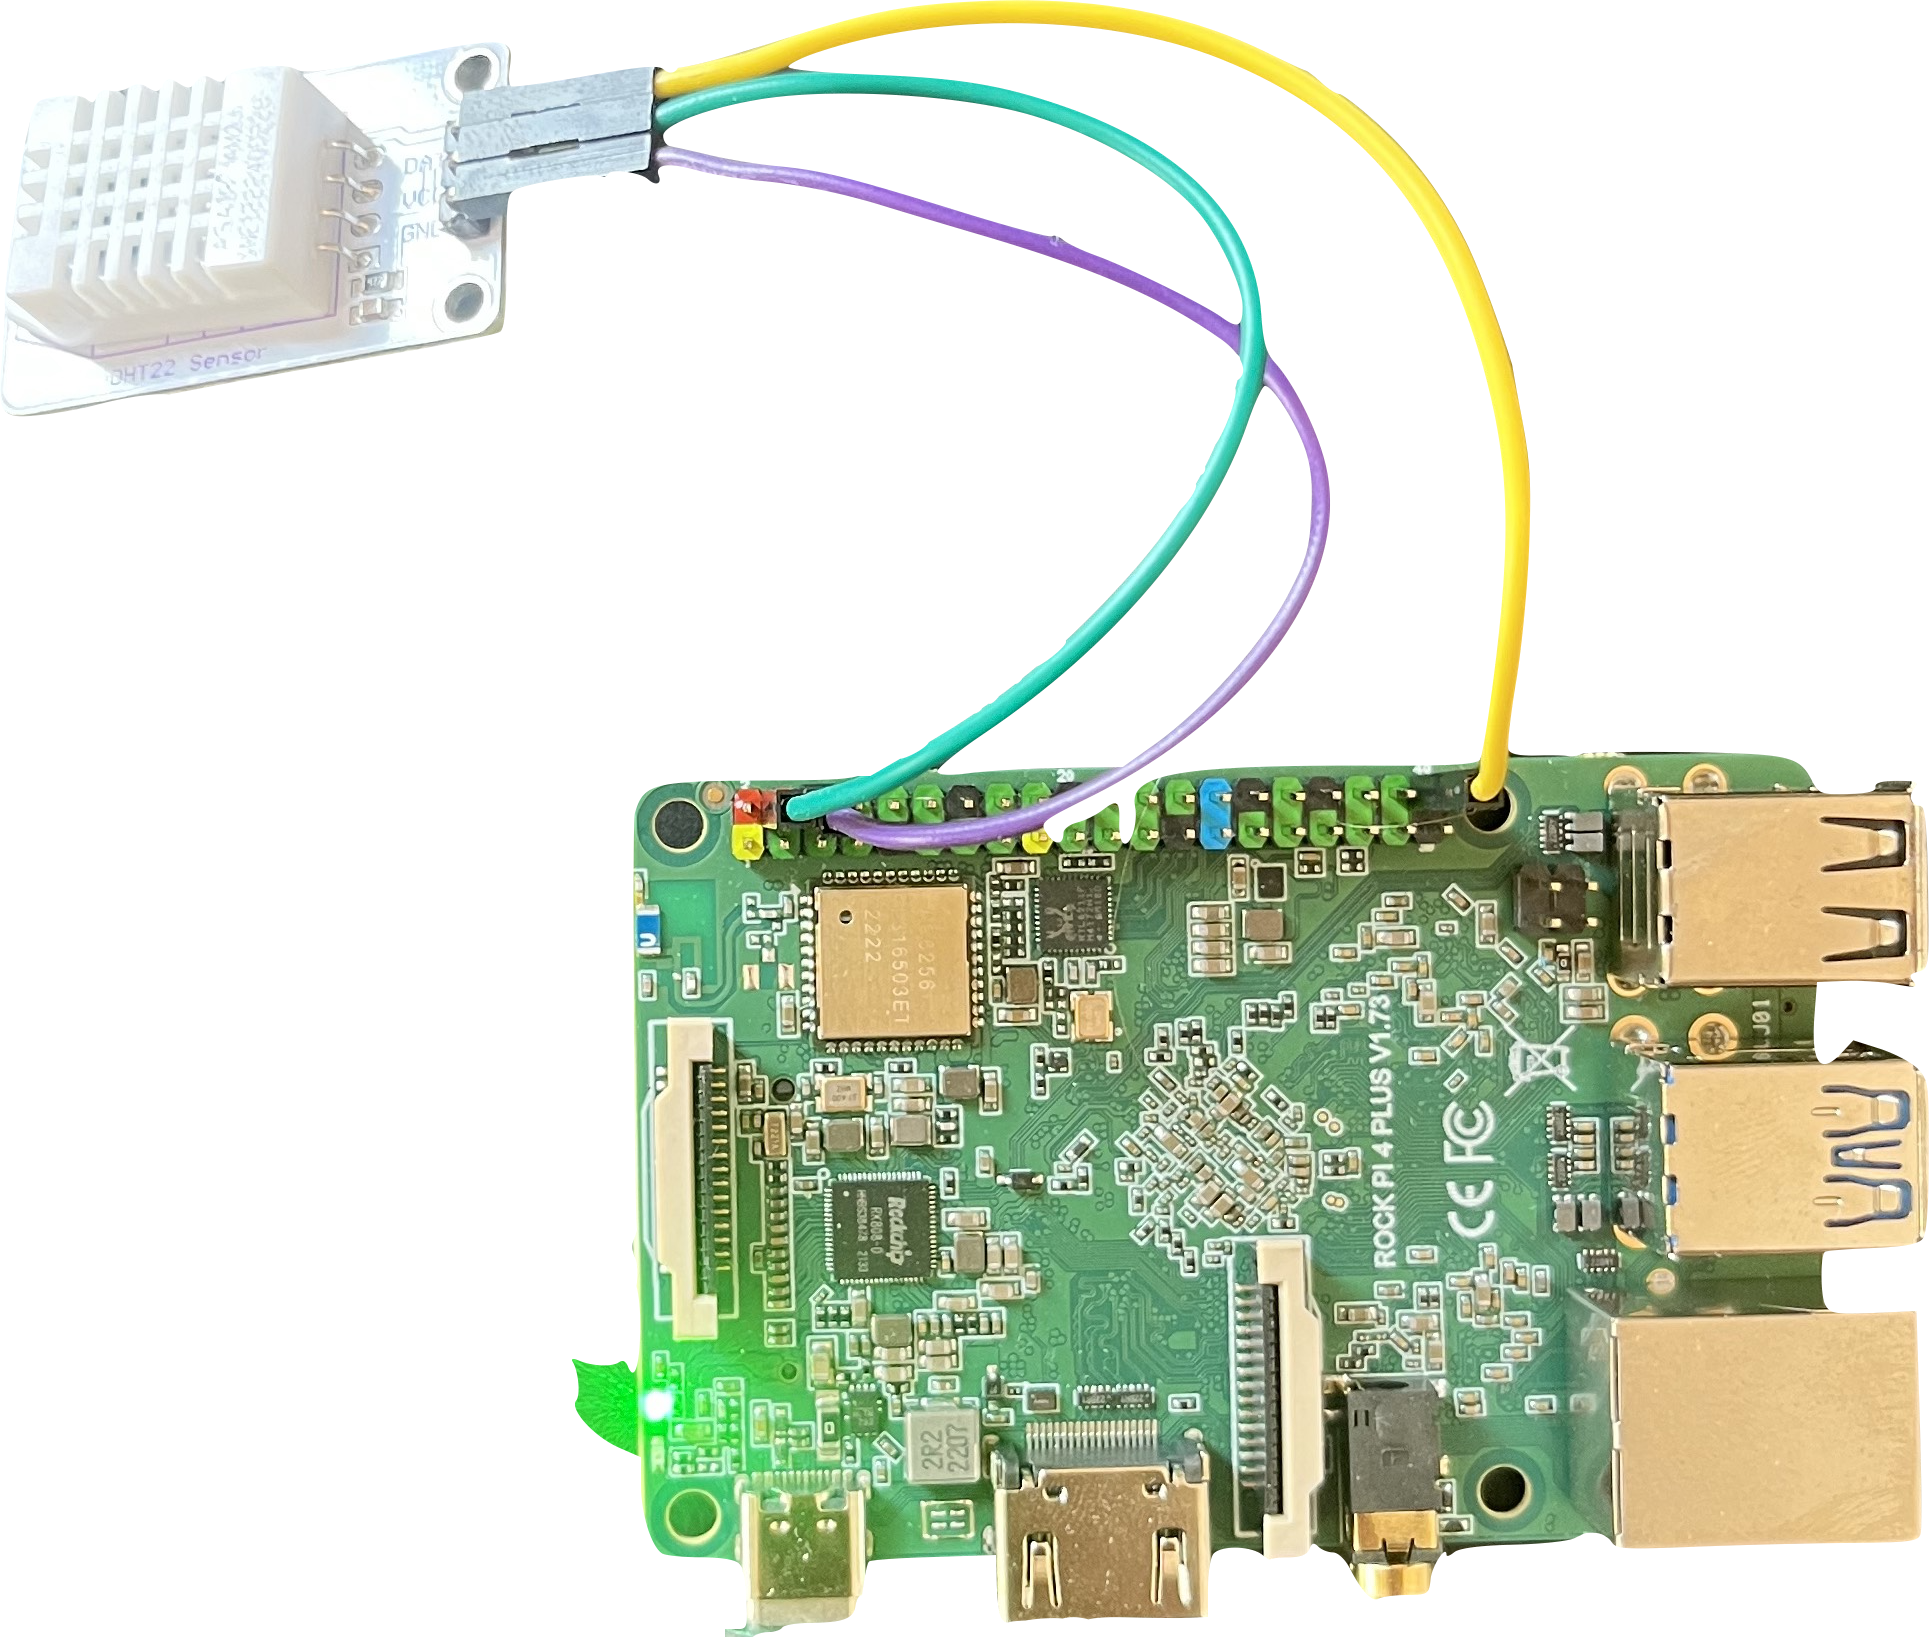
\includegraphics[width=0.49\textwidth]{resources/rock-pi.png}
    \caption{Rock Pi with a DHT-22 sensor} 
    \label{fig:rock-pi}
\end{figure}
Another major component of the system is the logging device used to monitor the environmental data during the transportation of the artwork. For this project, we used a Rock Pi \cite{rockpi4} with a DHT-22 \cite{dht22} sensor attached. (Figure \ref{fig:rock-pi})

The decision for this device and sensor is based on simplicity, flexibility, and low acquisition costs. The Rock Pi is compatible with the Linux operating system, making writing scripts using high-level programming languages like Python very simple. It also has \gls{gpio} support to connect the DHT-22 sensor easily. The sensor is capable of recording temperature and humidity data from the environment.

To read data from the DHT-22 sensor, we used an existing library called "Rockfruit Python DHT" \cite{rockfruitpythondht} that we adapted slightly to work with our board. The library provides a function with the signature \texttt{read\_retry(sensor, pin, retries=15, delay\_seconds=2)}. This method reads data from the DHT sensor of the specified type (in our case 22) on the specified \gls{gpio} pin. It returns a tuple of humidity (as a floating point value in percent) and temperature (as a floating point value in Celsius). 

The function will attempt to read multiple times (up to the specified retries) until a reading can be registered. If no reading can be registered after the number of retries, the function will return \texttt{(None, None)}. The default delay between retries is two seconds but can be overridden.

\begin{figure}[ht]
    \centering
    \begin{forest}
  for tree={
    font=\ttfamily,
    grow'=0,
    child anchor=west,
    parent anchor=south,
    anchor=west,
    calign=first,
    edge path={
      \noexpand\path [draw, \forestoption{edge}]
      (!u.south west) +(7.5pt,0) |- node[fill,inner sep=1.25pt] {} (.child anchor)\forestoption{edge label};
    },
    before typesetting nodes={
      if n=1
        {insert before={[,phantom]}}
        {}
    },
    fit=band,
    before computing xy={l=15pt},
  }
[artis-rockpi-logger
  [/Rockfruit\_Python\_DHT
  ]
  [artis\_api.py
  ]
  [authenticator.py
  ]
  [logging\_script.py
  ]
  [violation\_script.py
  ]
]
\end{forest}    
    \caption{Logger directory structure}
    \label{fig:artis-logger-filetree}
\end{figure}

\subsection{Code}
\lstinputlisting[
    language=Python,
    caption=Temperature and humidity logging loop in \texttt{logging\_script.py},
    label=lst:loggingscript,
    float
]{codesnippets/logging_script.py}

In Listing \ref{lst:loggingscript}, you can see that the script is executing the \texttt{read\_retry} function in an endless loop, and whenever the reading has been successful, it stores the data along with a timestamp of the reading in seconds and a readable format in a local database.

The logger contains a second important script which is run simultaneously. The \texttt{violation\_script.py} is executed with the predefined temperature and humidity thresholds and the corresponding artwork \gls{id}.

\lstinputlisting[
    language=bash,
    caption=Executing the \texttt{violation\_script.py},
    label=lst:violationscript,
    xleftmargin=2cm,
    xrightmargin=2cm
]{codesnippets/violation_script.py}

This script contains another while loop that continuously checks for new entries in the database and evaluates whether the threshold has been exceeded. If there has been either a temperature or humidity violation, the script calls the corresponding method to call the \texttt{ARTIS} server \gls{api}. These methods are defined in the \texttt{artis\_api.py} file.

To authenticate to the \gls{api}, the logger follows the same authentication flow illustrated in Figure \ref{fig:auth_flow}. The methods used to send the authentication requests and sign the challenge message are defined in the \texttt{authenticator.py} file.

\clearpage
\section{artis-frontend}
The last component of the system is the user interface. It is a single-page application built with React \cite{react} and TypeScript. The styling is done with Tailwind CSS \cite{tailwindcss}. These technologies were selected due to the author's prior experience. Theoretically, the user interface is not required to interact with the system. However, simple authentication is a large benefit of the user interface. Its integration with Metamask \cite{metamask} enables a seamless login and authentication flow. From a code perspective, thirdweb \cite{thirdweb} is used to access the \gls{api} of Metamask. A short demo of the user interface can be viewed here GitHub\footnote{\href{https://artis-project.github.io/artis-thesis/frontend-demo.mov}{https://artis-project.github.io/artis-thesis/frontend-demo.mov}}

\begin{figure}[h]
    \centering
    \begin{subfigure}{\textwidth}
        \centering
        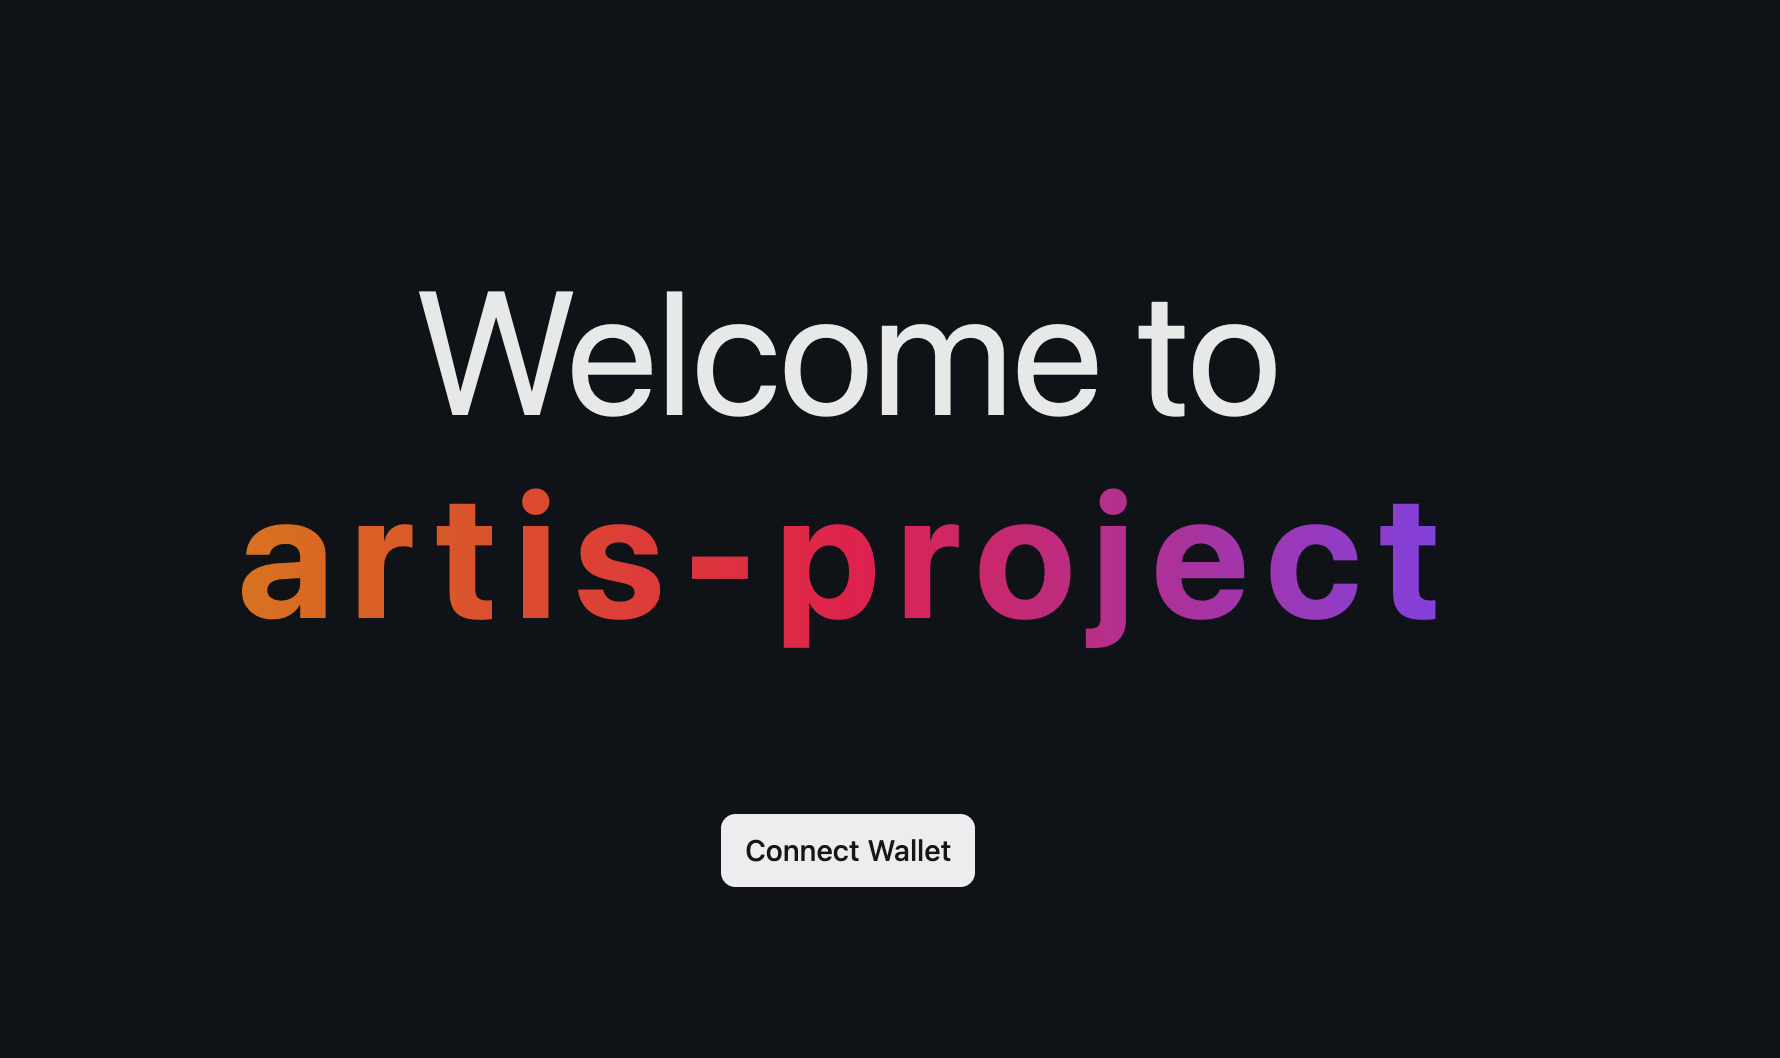
\includegraphics[width=0.8\textwidth]{resources/frontend_screenshots/welcome_screen.png}
        \caption{Welcome Screen}
        \label{fig:welcome_screen}
        \vspace*{2mm}
    \end{subfigure}
    \begin{subfigure}{\textwidth}
        \centering
        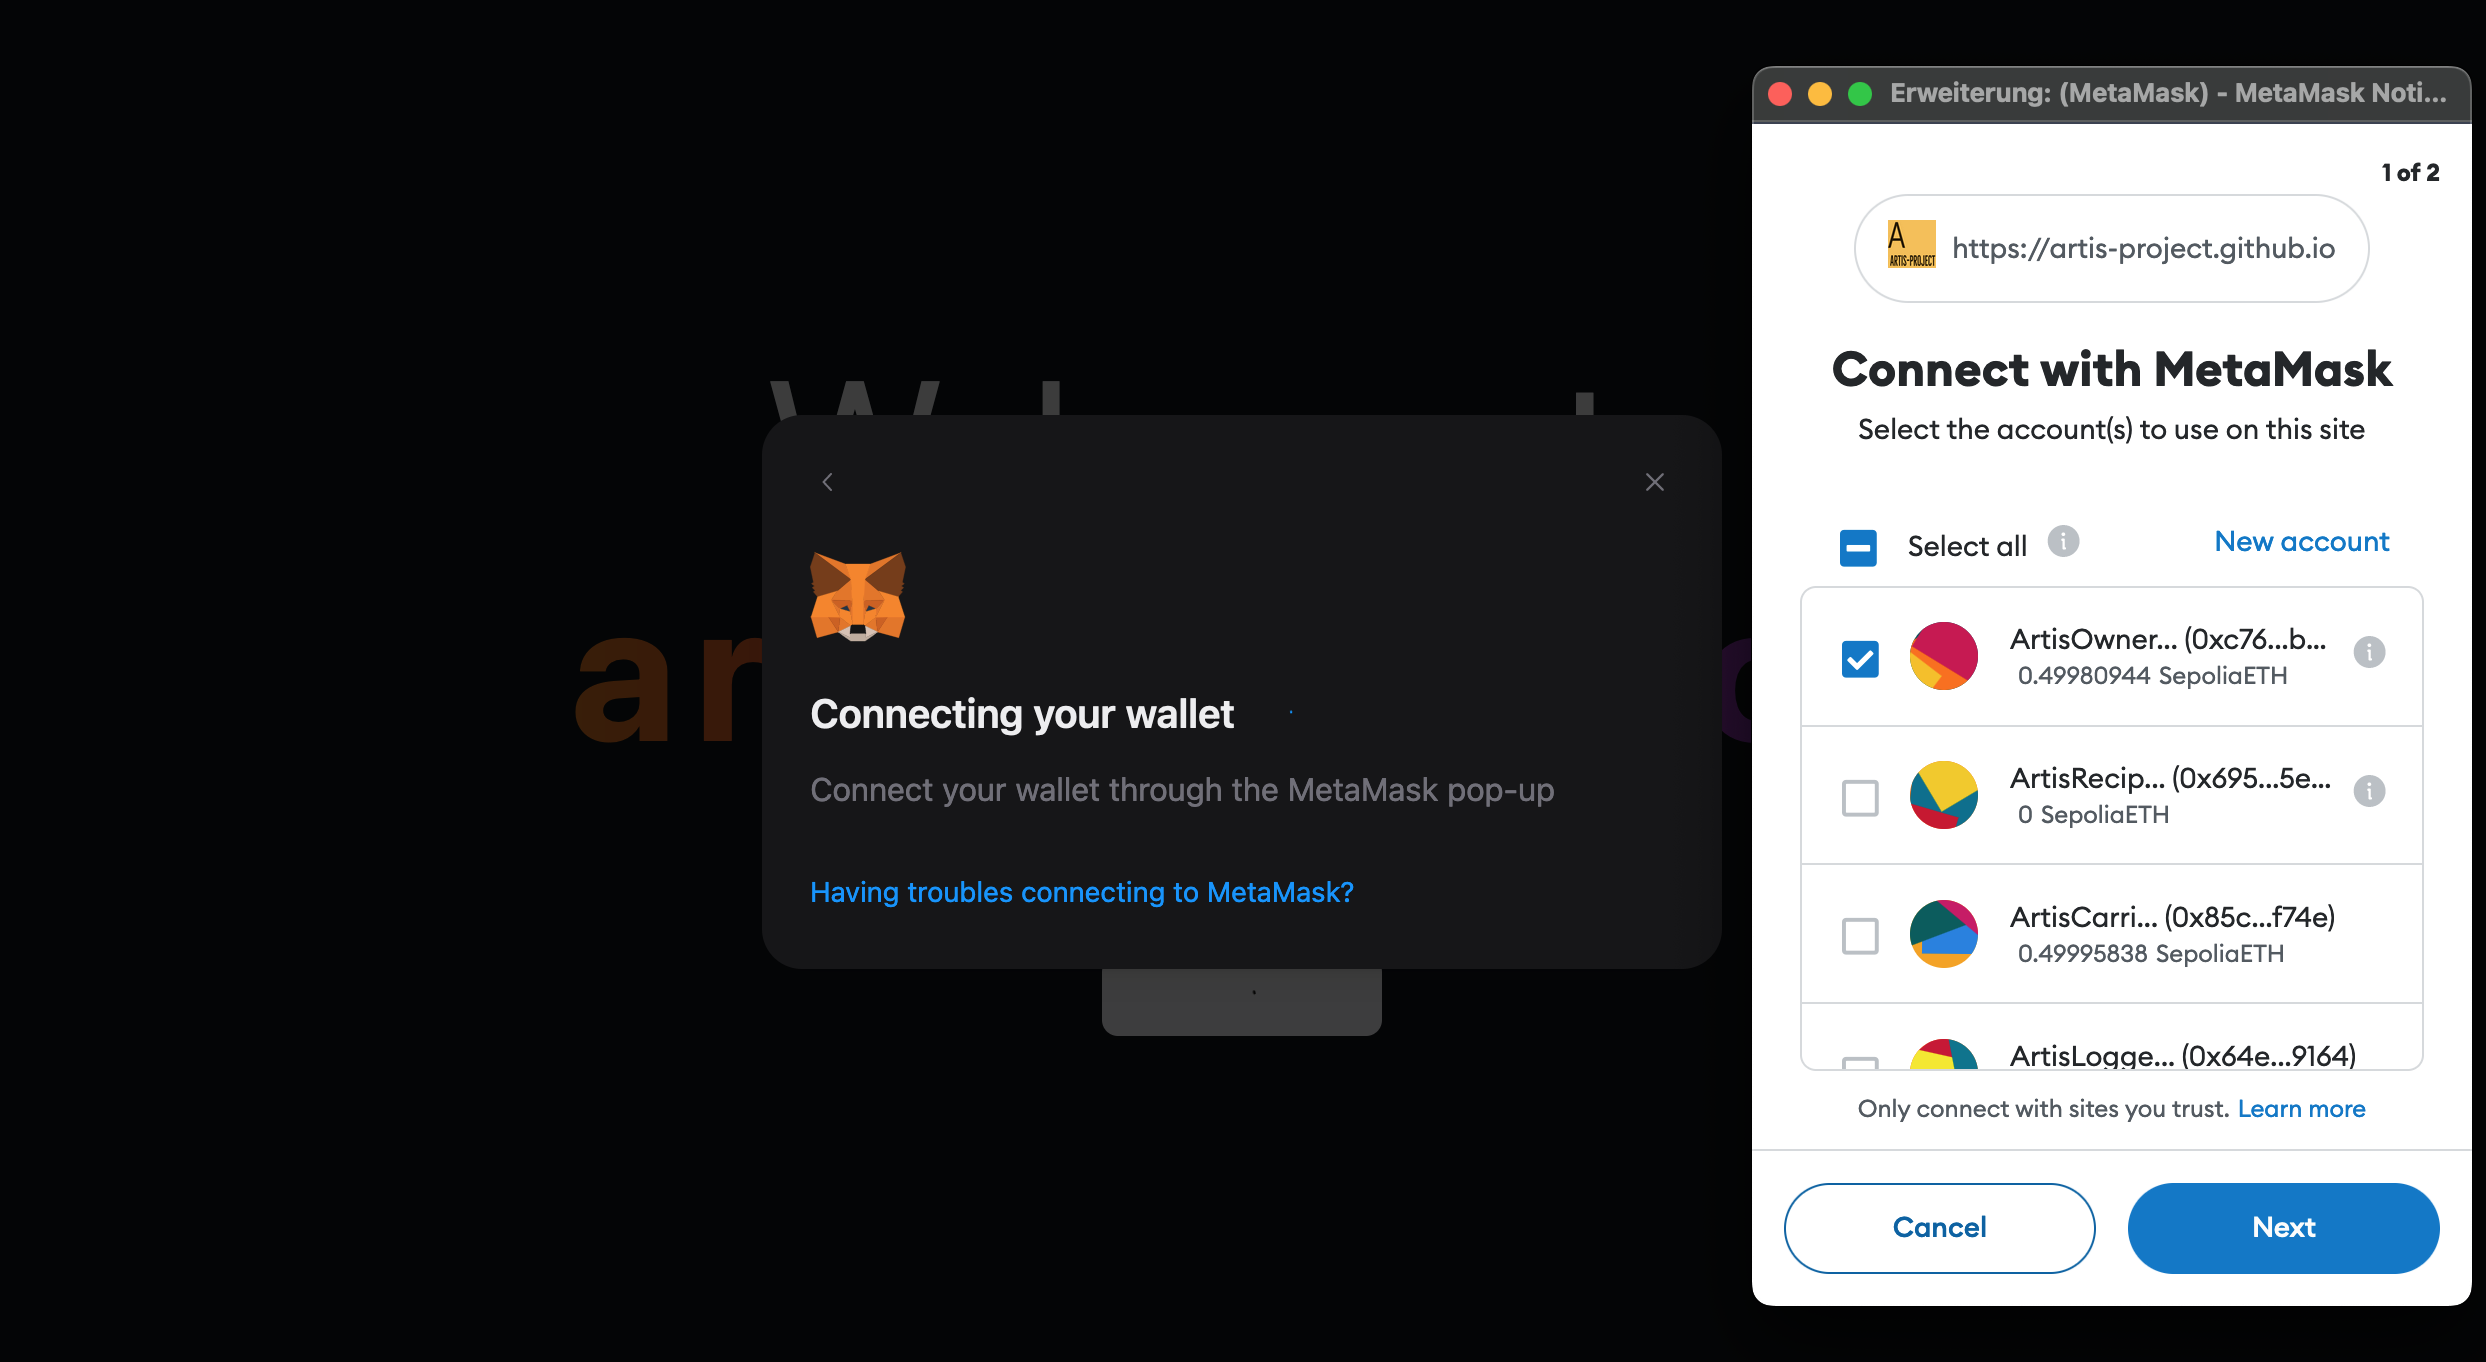
\includegraphics[width=0.8\textwidth]{resources/frontend_screenshots/connecting_wallet.png}
        \caption{Connecting to Metamask}
        \label{fig:connecting_metamask}
    \end{subfigure}
\end{figure}

An unauthenticated user first lands on this welcome page with a button to connect the website to Metamask as shown in Figure \ref{fig:welcome_screen}. After pressing the button, Metamask opens a pop-up to select an account to connect to the website (Figure \ref{fig:connecting_metamask}). Finally, the button label changes to "Sign in" and as soon as the user presses the button again, a signature request is sent to the server. The message visible on the pop-up in Figure \ref{fig:sign_in} is a message constructed from the response of the POST \texttt{/auth/payload} request.

Once the user signs this message, the signature is sent back to the server, validated, and an authentication token is issued. The user is now logged in and can see all the artworks by their \glspl{id} that are associated with the logged-in account (Figure \ref{fig:artworks_page}).

\begin{figure}[h!]
    \ContinuedFloat
    \begin{subfigure}{\textwidth}
        \centering
        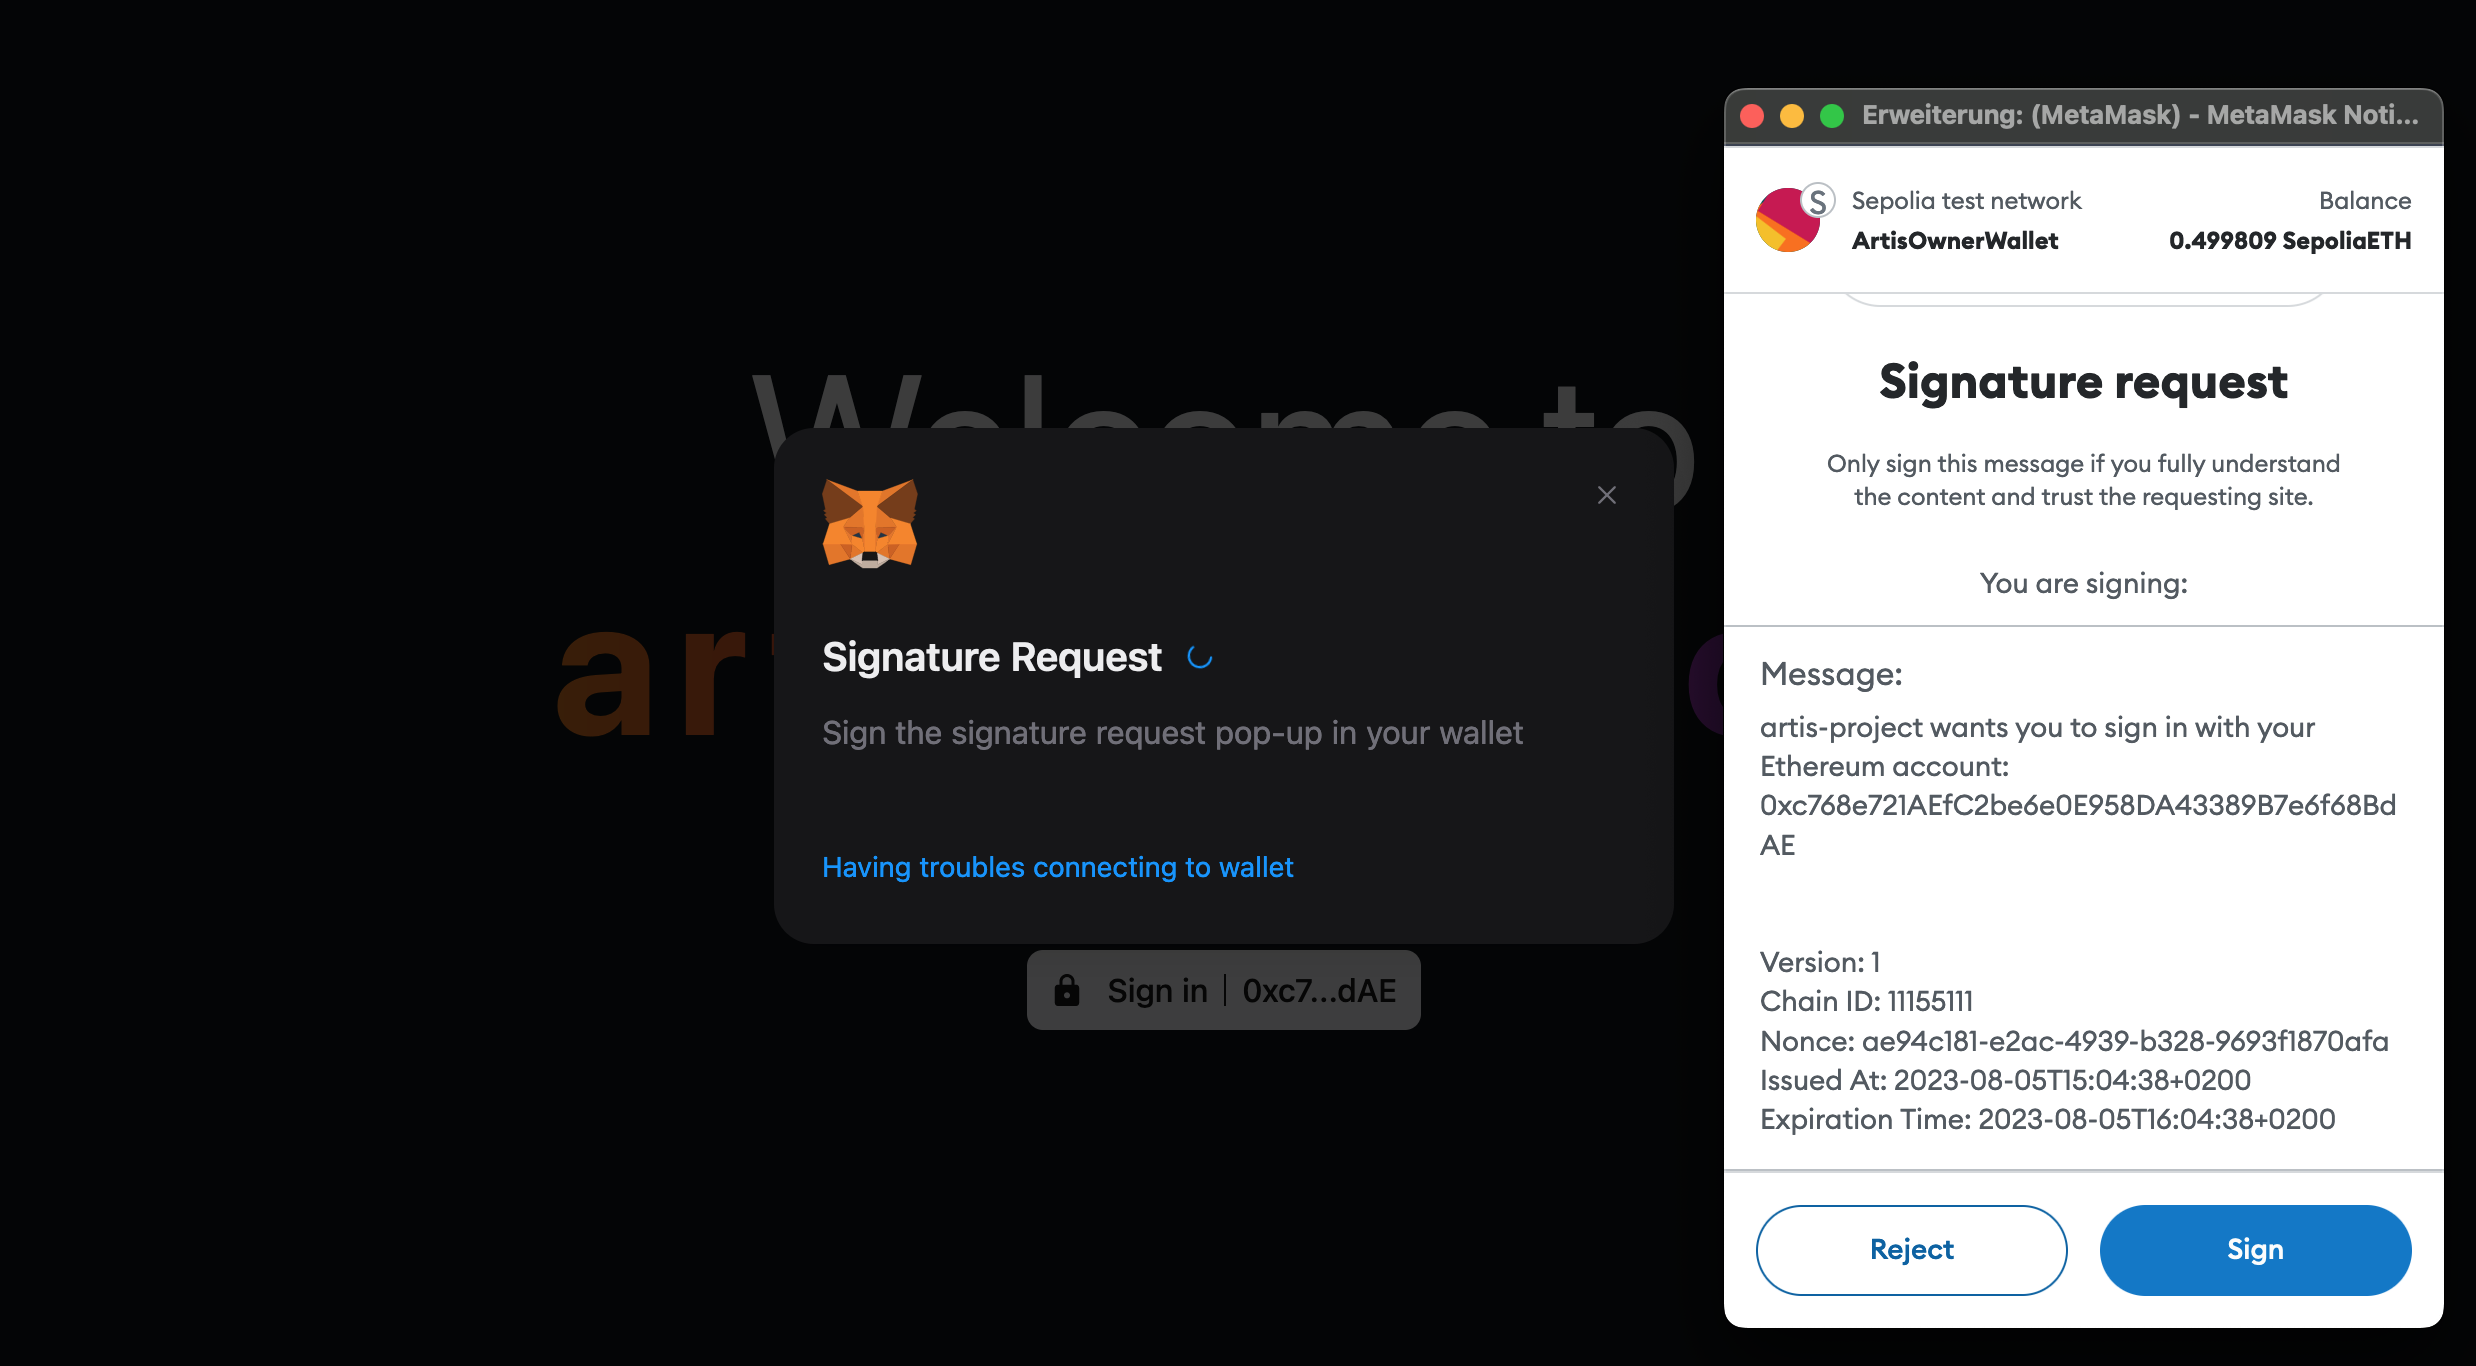
\includegraphics[width=0.8\textwidth]{resources/frontend_screenshots/sign_in.png}
        \caption{Sign in request}
        \label{fig:sign_in}
        \vspace*{2mm}
    \end{subfigure}
\end{figure}

\begin{figure}[h]
    \ContinuedFloat
    \centering
    \begin{subfigure}{\textwidth}
        \centering
        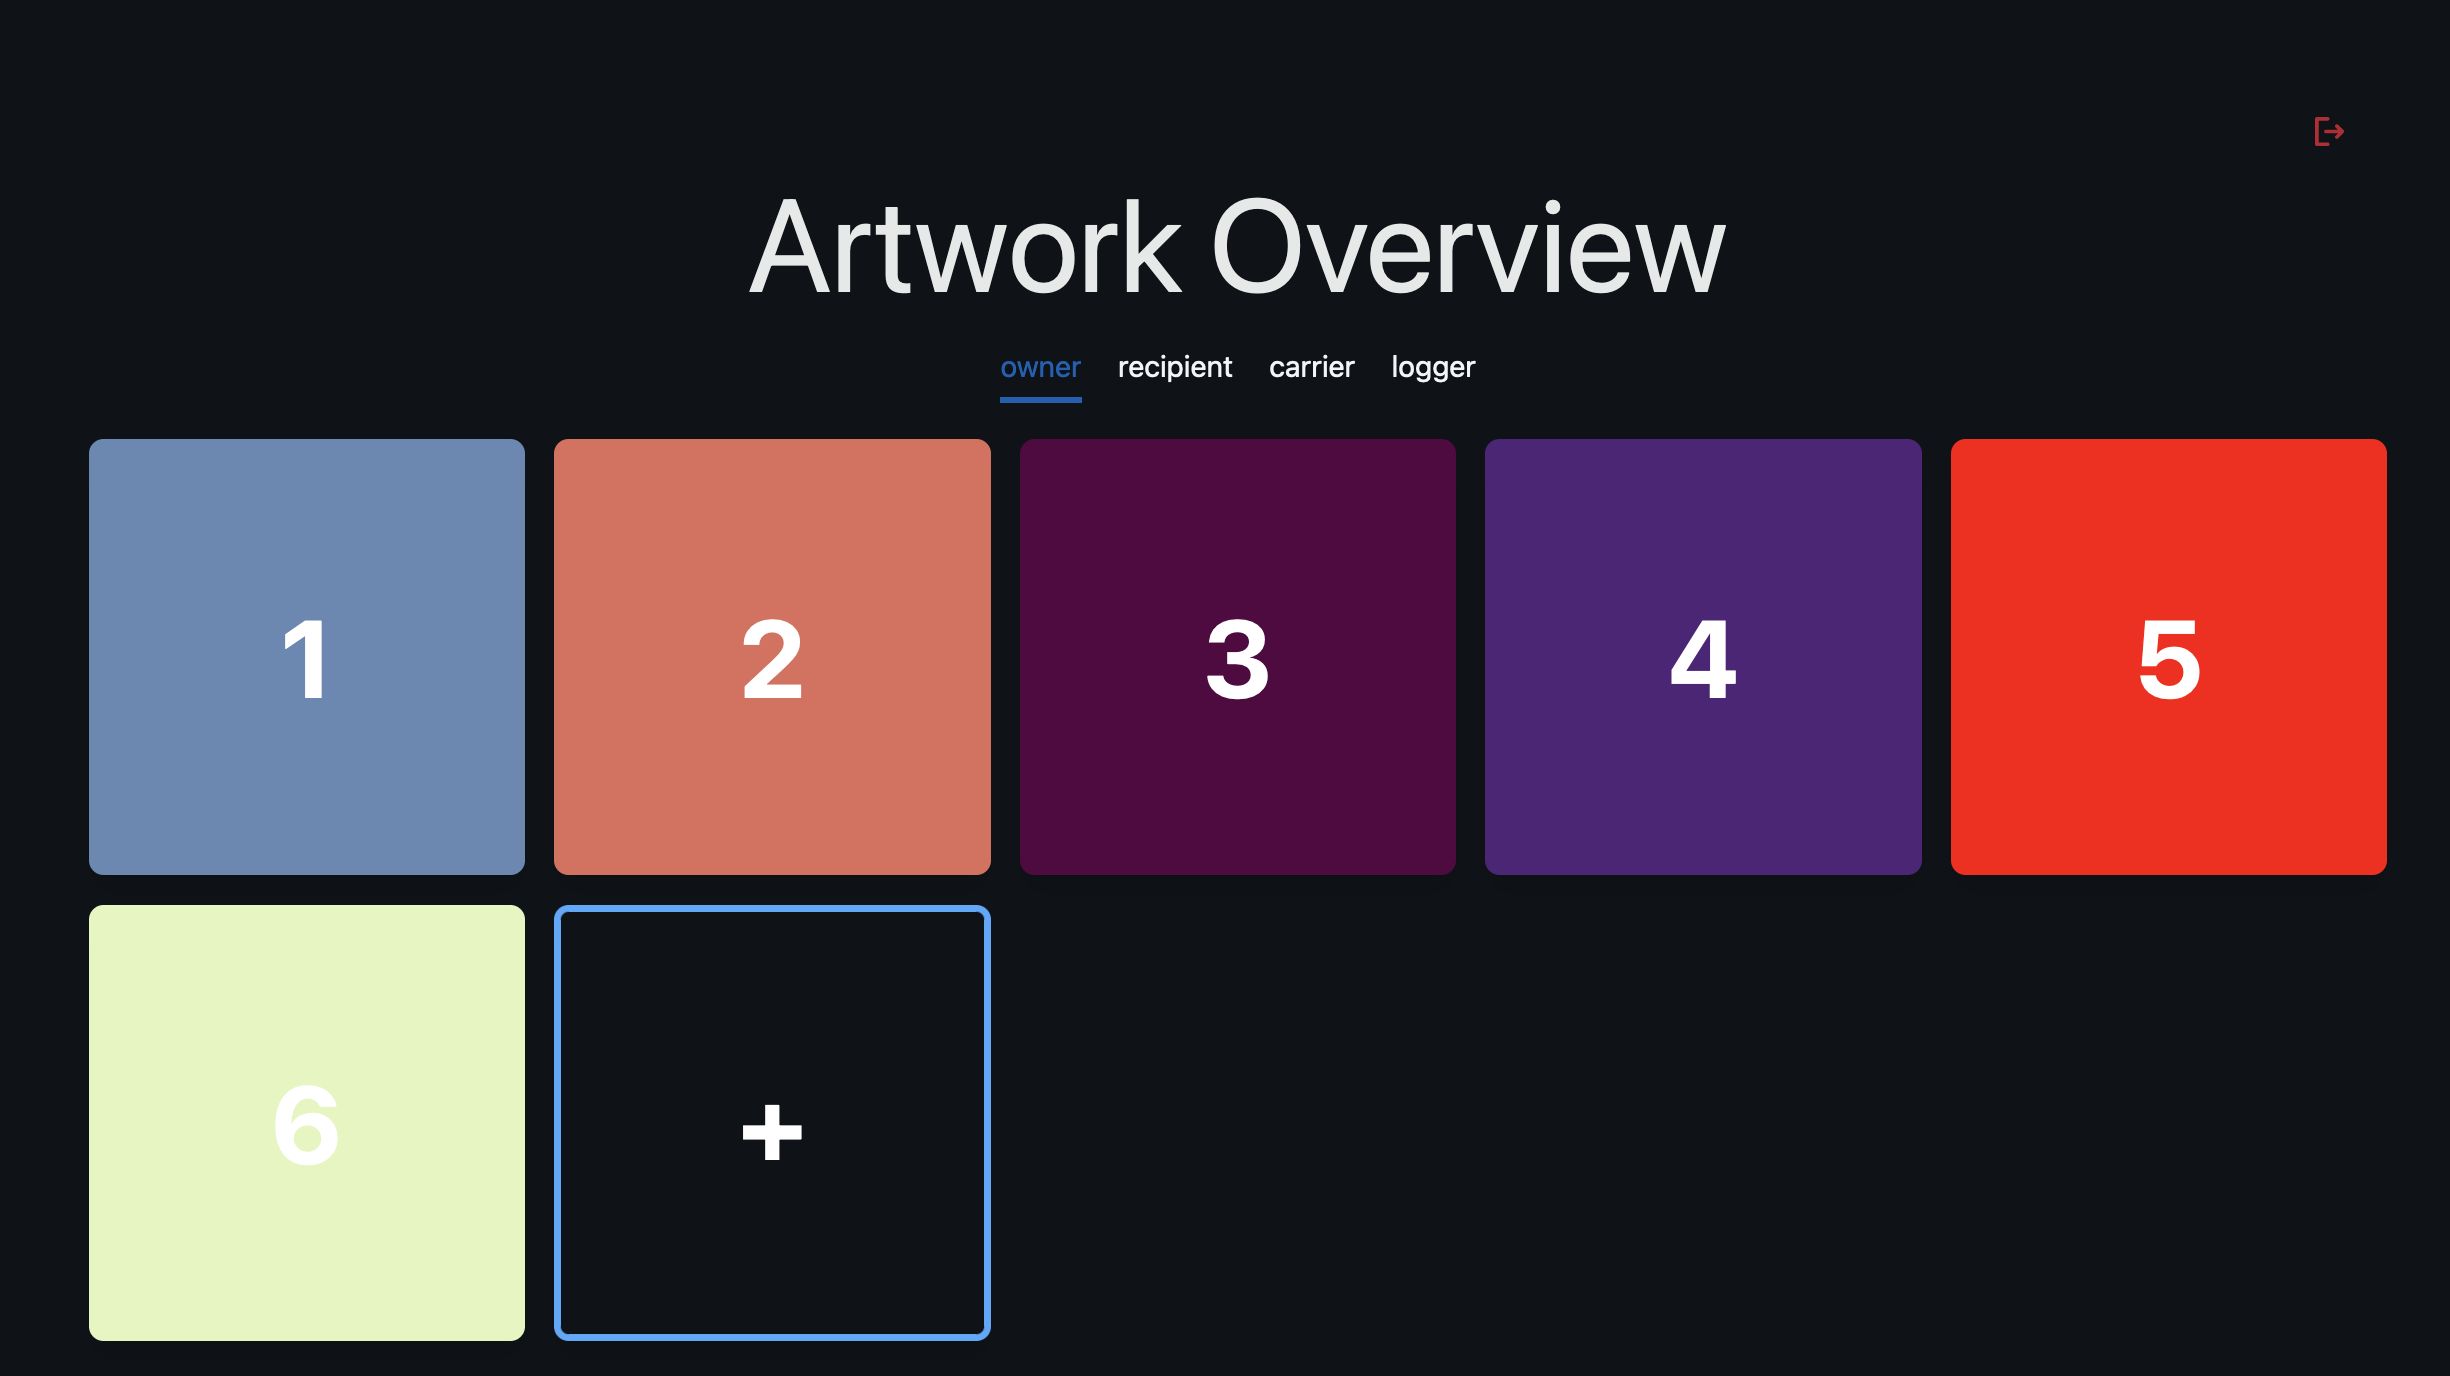
\includegraphics[width=0.8\textwidth]{resources/frontend_screenshots/artworks_page.png}
        \caption{Artworks page}
        \label{fig:artworks_page}
    \end{subfigure}
    \caption{Sign in process}
    \label{fig:sign_in_process}
\end{figure}

The artwork page shows a colorful tile representing an artwork. Each tile is labeled with the corresponding artwork \gls{id}. The tabs on the top can be selected to view all the artworks where the account is registered \textit{e.g.} the user might be the artwork owner $1$ but the recipient $2$. 

\begin{figure}
    \centering
    \begin{minipage}{0.45\textwidth}
        \centering
        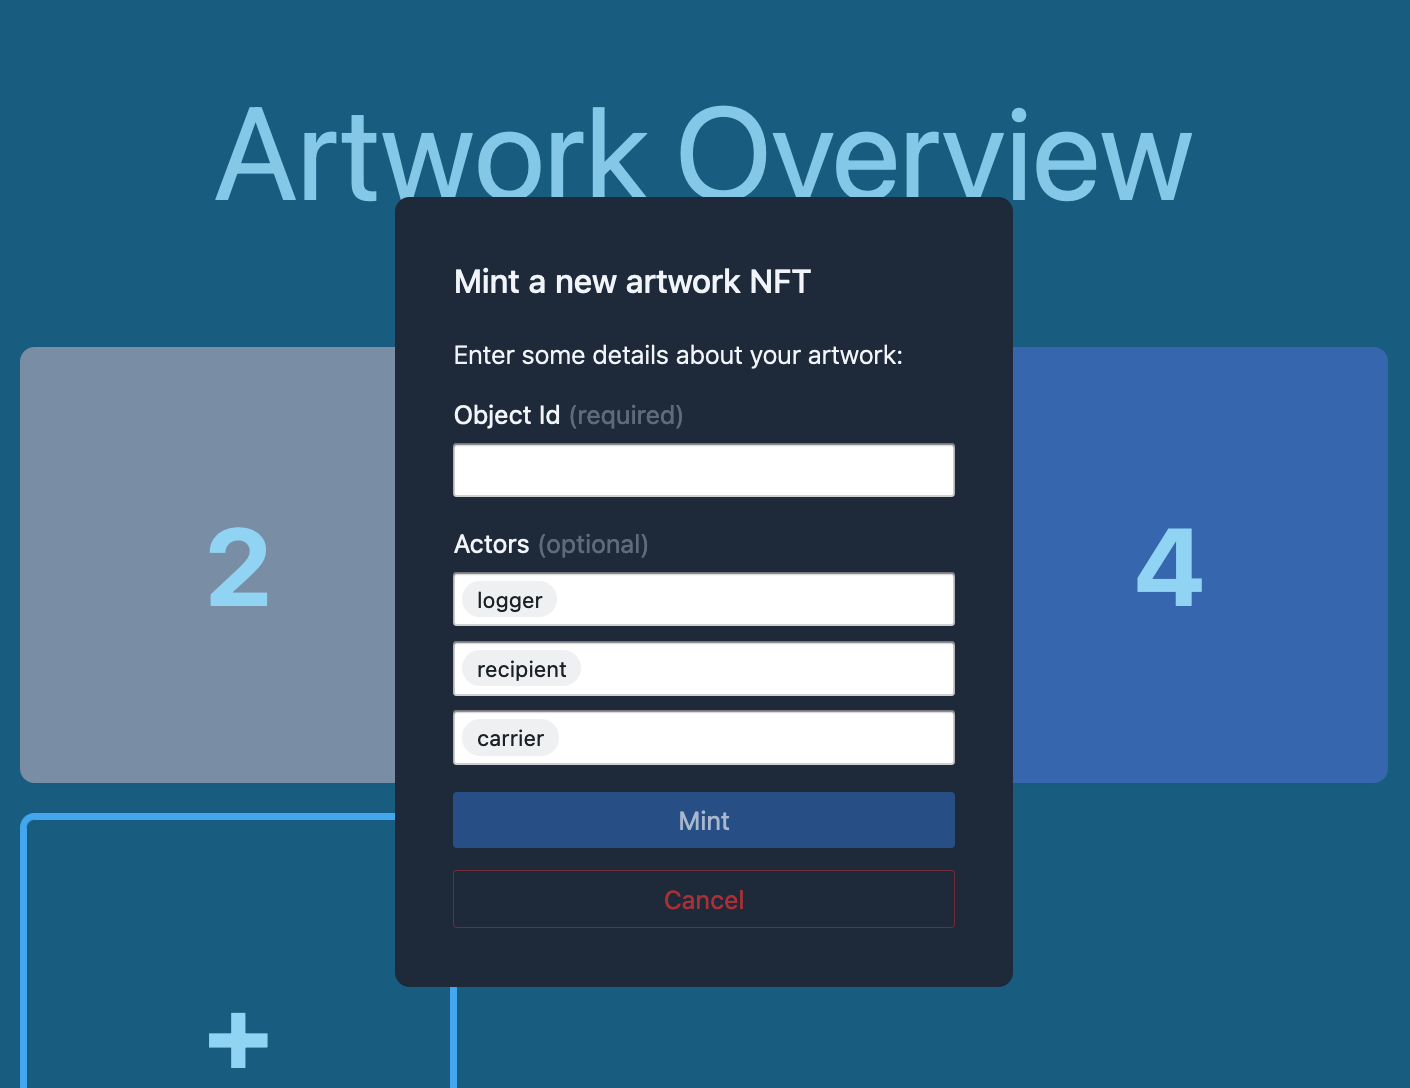
\includegraphics[height=0.4\textheight]{resources/frontend_screenshots/mint_modal.png}
        \caption{Artwork mint modal}
        \label{fig:mint_modal}
    \end{minipage}\hfill
    \begin{minipage}{0.45\textwidth}
        \centering
        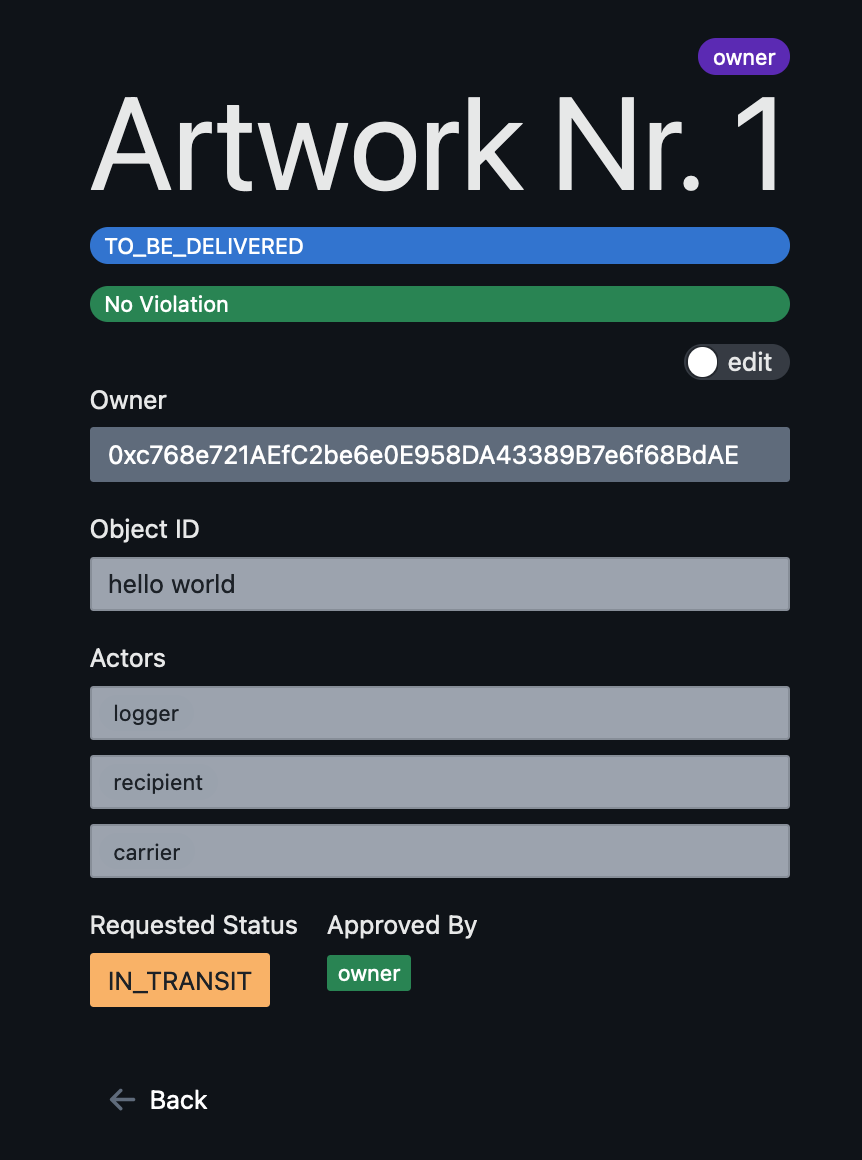
\includegraphics[height=0.4\textheight]{resources/frontend_screenshots/artwork_details.png}
        \caption{Artwork detail view}
        \label{fig:artwork_detail}
    \end{minipage}
\end{figure}

To create a new artwork \gls{nft}, the user can click on the transparent tile at the bottom. This will open up a modal where the user can enter details about the artwork (Figure \ref{fig:mint_modal}). To view more details about an existing artwork the user can click on a tile to open up the detail view shown in Figure \ref{fig:artwork_detail}. This view displays important information like the status of the artwork, the role the user is registered as, and the timestamp of the most recent violation if any occurred. Further, the user can edit values by switching on the edit mode with the switch on the top right.  

